\section{多种性能指标测试评估}

\subsection{NPUcore系统调用性能分析}

NPUcore性能得分如下:

\begin{table}[H]
    \centering
    \begin{tabular}{|l|r|}
        \hline
        测例 & 耗时 \\
        \hline
        b\_malloc\_tiny2 (0) & 0.005085920 \\
        \hline
        b\_malloc\_big2 (0) & 0.028311200 \\
        \hline
        b\_malloc\_thread\_stress (0) & 0.066339520 \\
        \hline
        b\_string\_strstr ("abcdefghijklmnopqrstuvwxyz") & 0.011712000 \\
        \hline
        b\_string\_strstr ("azbycxdwevfugthsirjqkplomn") & 0.017838240 \\
        \hline
        b\_string\_strstr ("aaaaaaaaaaaaaacccccccccccc") & 0.011262640 \\
        \hline
        b\_string\_strstr ("aaaaaaaaaaaaaaaaaaaaaaaaac") & 0.010942000 \\
        \hline
        b\_string\_strstr ("aaaaaaaaaaaaaaaaaaaaaaaaaaaaaaaac") & 0.013523120 \\
        \hline
        b\_string\_memset (0) & 0.009740400 \\
        \hline
        b\_string\_strchr (0) & 0.011392640 \\
        \hline
        b\_string\_strlen (0) & 0.009787360 \\
        \hline
        b\_pthread\_createjoin\_serial1 (0) & 0.439336960 \\
        \hline
        b\_pthread\_createjoin\_serial2 (0) & 0.426977760 \\
        \hline
        b\_pthread\_create\_serial1 (0) & 0.476990480 \\
        \hline
        b\_pthread\_uselesslock (0) & 0.060514480 \\
        \hline
        b\_utf8\_bigbuf (0) & 0.032511520 \\
        \hline
        b\_utf8\_onebyone (0) & 0.091743280 \\
        \hline
        b\_stdio\_putcgetc (0) & 0.439399360 \\
        \hline
        b\_stdio\_putcgetc\_unlocked (0) & 0.426097680 \\
        \hline
        b\_regex\_compile ("(a|b|c)*d*b") & 0.057043200 \\
        \hline
    \end{tabular}
    \caption{Npucore的libc-bench}
\end{table}

\begin{table}[H]
    \centering
    \begin{tabular}{|l|r|}
        \hline
        \textbf{测试名称} & \textbf{数值} \\
        \hline
        Unixbench DHRY2 test(lps) & 61405230 \\
        \hline
        Unixbench WHETSTONE test(MFLOPS) & 1269.670 \\
        \hline
        Unixbench SYSCALL test(lps) & 222615 \\
        \hline
        Unixbench CONTEXT test(lps) & 168113 \\
        \hline
        Unixbench PIPE test(lps) & 413979 \\
        \hline
        Unixbench SPAWN test(lps) & 64394 \\
        \hline
        Unixbench EXECL test(lps) & 73597 \\
        \hline
        Unixbench ARITHOH test(lps) & 7032261867 \\
        \hline
        Unixbench SHORT test(lps) & 179342297 \\
        \hline
        Unixbench INT test(lps) & 179660281 \\
        \hline
        Unixbench LONG test(lps) & 179644882 \\
        \hline
        Unixbench FLOAT test(lps) & 178725171 \\
        \hline
        Unixbench DOUBLE test(lps) & 179034748 \\
        \hline
        Unixbench HANOI test(lps) & 677685 \\
        \hline
        Unixbench EXEC test(lps) & 39493 \\
        \hline
    \end{tabular}
    \caption{Npucore的Unixbench测试结果}
    \label{Npucore的Unixbench测试结果}
\end{table}


\subsection{其他内核系统调用性能分析}


\subsubsection{Titanix}


\subsubsection{PLNTRY}

首先,从https://gitlab.eduxiji.net/PLNTRY/OSKernel2023-umi/-/blob/comp3-coverage地址处克隆仓库,
切换到master分支。将比赛提供的镜像文件复制到OSKernel2023-umi/third-party/img文件目录下,
命名为sdcard-comp2.img,在主文件目录下make all,make run即可运行该kernel。
注意,所有的测试结果不直接在终端显示,而在debug/ qemu.log 中显示。

下面将展示PLNTRY的性能得分情况,并与npucore进行简单的对比。

\begin{table}[H]
    \centering
    \begin{tabular}{|l|r|}
        \hline
        测例 & 耗时 \\
        \hline
        b\_malloc\_sparse (0) & 0.749882000 \\
        \hline
        b\_malloc\_bubble (0) & 0.795564000 \\
        \hline
        b\_malloc\_tiny1 (0) & 0.020421000 \\
        \hline
        b\_malloc\_tiny2 (0) & 0.013895000 \\
        \hline
        b\_malloc\_big1 (0) & 0.205780000 \\
        \hline
        b\_malloc\_big2 (0) & 0.159222000 \\
        \hline
        b\_malloc\_thread\_stress (0) & 0.065488000 \\
        \hline
        b\_malloc\_thread\_local (0) & 0.057541000 \\
        \hline
        b\_string\_strstr ("abcdefghijklmnopqrstuvwxyz") & 0.014606000 \\
        \hline
        b\_string\_strstr ("azbycxdwevfugthsirjqkplomn") & 0.022971000 \\
        \hline
        b\_string\_strstr ("aaaaaaaaaaaaaacccccccccccc") & 0.014078000 \\
        \hline
        b\_string\_strstr ("aaaaaaaaaaaaaaaaaaaaaaaaac") & 0.013603000 \\
        \hline
        b\_string\_strstr ("aaaaaaaaaaaaaaaaaaaaaaaaaaaaaaaac") & 0.017628000 \\
        \hline
        b\_string\_memset (0) & 0.012005000 \\
        \hline
        b\_string\_strchr (0) & 0.014630000 \\
        \hline
        b\_string\_strlen (0) & 0.012690000 \\
        \hline
        b\_pthread\_createjoin\_serial1 (0) & 1.048143000 \\
        \hline
        b\_pthread\_createjoin\_serial2 (0) & 1.020008000 \\
        \hline
        b\_pthread\_create\_serial1 (0) & 2.689056000 \\
        \hline
        b\_pthread\_uselesslock (0) & 0.078151000 \\
        \hline
        b\_utf8\_bigbuf (0) & 0.037977000 \\
        \hline
        b\_utf8\_onebyone (0) & 0.117029000 \\
        \hline
        b\_stdio\_putcgetc (0) & 0.361184000 \\
        \hline
        b\_stdio\_putcgetc\_unlocked (0) & 0.339361000 \\
        \hline
        b\_regex\_compile ("(a|b|c)*d*b") & 0.075878000 \\
        \hline
        b\_regex\_search ("(a|b|c)*d*b") & 0.086110000 \\
        \hline
        b\_regex\_search ("a\{25\}b") & 0.256301000 \\
        \hline
    \end{tabular}
    \caption{libc-bench}
\end{table}

\begin{table}[H]
    \centering
    \begin{tabular}{|l|r|}
    \hline
        测试项 & 得分 \\
        \hline
        DHRY2 (lps) & 48523418 \\
        \hline
        WHETSTONE (MFLOPS) & 1014.102 \\
        \hline
        SYSCALL (lps) & 547678 \\
        \hline
        CONTEXT (lps) & 42416 \\
        \hline
        PIPE (lps) & 802449 \\
        \hline
        SPAWN (lps) & 13586 \\
        \hline
        ARITHOH (lps) & 5541357804 \\
        \hline
        SHORT (lps) & 140413305 \\
        \hline
        INT (lps) & 140311940 \\
        \hline
        LONG (lps) & 140287530 \\
        \hline
        FLOAT (lps) & 142030413 \\
        \hline
        DOUBLE (lps) & 141484435 \\
        \hline
        HANOI (lps) & 536762 \\
    \hline
    \end{tabular}
    \caption{plntry的Unixbench}
    \label{tab:unixbench}
\end{table}

通过比较Npucore和plntry的libc-bench和Unix-bench可以发现,在libc-bench中,Npucore的和plntry的所耗时间比较相似,这与测例的相对简单有比较大的关系。但是在Unix-bench中,plntry的部分性能得分优于Npucore。例如SYSCALL (lps),CONTEXT (lps),PIPE (lps),当然Npucore也有比plntry表现更良好的测试项,比如DHRY2 test(lps), SPAWN test(lps)等。

"syscall" 测试是一个基准测试,用于评估系统在执行系统调用(syscalls)时的性能。系统调用是操作系统提供给用户空间程序访问操作系统内核功能的接口。
这个测试旨在测量系统在执行各种系统调用时的效率和速度。UnixBench会执行一系列常见的系统调用,比如文件操作、进程控制、内存管理等,然后测量系统在执行这些调用时所需的时间和性能。
"syscall" 测试的结果以每秒钟能够执行的系统调用数量(lps - syscalls per second)作为单位,因此其结果值越高表示系统在处理系统调用时的效率越高,执行系统调用的能力也就越强。

UnixBench中的 "CONTEXT" 测试是用来评估系统在上下文切换方面的性能。上下文切换是操作系统在多任务环境中切换执行不同进程或线程时所需的过程。
"CONTEXT" 测试测量系统在进行上下文切换时的效率,它涉及将处理器从一个进程或线程切换到另一个的能力。在多任务系统中,上下文切换是一种常见操作,而系统的性能可能会受到其影响。
测试结果以每秒钟能够完成的上下文切换数量(lps - context switches per second)作为单位。因此,较高的数值表示系统在处理上下文切换时更有效率,能够更快地在不同的进程或线程之间进行切换。

"spawn" 测试是一个基准测试,用于评估系统在并发进程创建和销毁方面的性能。该测试模拟了系统同时启动多个进程的情况,然后检查系统在这种高并发情况下的性能表现。
"spawn" 测试通常会创建许多子进程,然后立即销毁它们,以测试系统处理这些操作的速度和效率。这个测试可以显示系统在处理并发任务时的能力,因为进程的创建和销毁在某些应用场景下可能是非常常见的操作。
UnixBench中的 "spawn" 测试的结果以每秒钟能够创建和销毁的进程数(lps - processes per second)作为单位,因此其结果值越高表示系统在这个方面的性能越好。


性能优秀的原因:
\begin{itemize}
    \item 内存管理:在页帧管理实现写时复制策略和通用 IO 缓
存,减少 IO 设备访问次数。
在地址空间管理实现懒分配策略,提高内存.

在设计UMI的页帧管理模块的部分,借鉴 Fuchsia 设计了一套 RAII 的基于二叉树形的数据结构。
每个节点逻辑上是其父节点的一个切片,有标志指示是否拥有写时复制(CoW)特性。
页帧通过引用计数和缓存状态的更新在树形结构中复制和流动。例如在提交页帧的时候,
依次从自身的哈希表、父节点的哈希表、I/O 后端读写、新清零页的顺序来依次访问并提
交页帧。

通过如上说明可以看到,Phys 结构体可以作为任意读写+寻址的后端的页缓存,包
括普通文件、块设备等。这样,虽然缺乏了一些特定场景的优化,可以避免重复的页缓
存代码。并且由于写时复制和懒分配两个特性,任何涉及到内存分配的场景都会获得对应的
性能提升。同时,每个节点可以实现同时读写页帧,在不浪费页帧的情况下提升页缓存的并
发性。
    \item 线程管理与调度:使用细粒度锁和 Rust 所有权系统管理线程
的本地状态和信息
支持软抢占和任务窃取的 SMP 多核调度器
基于有栈协程模式的特权级切换

传统的操作系统往往采用有栈协程将任务的调用栈和上下文分开保存,通过汇编代码手动
切换函数调用栈来进行任务切换。每个任务的调用栈都会有一定的内存浪费(空闲),并都
会有栈溢出风险。

而无栈协程则将任务的信息同一保存成状态机,统一存放在堆上,由执行器通过更改指
针来切换执行的任务。从图中我们可以发现,调用栈仅与每个执行器一一绑定,一定程度上
减少了内存浪费、降低栈溢出风险。

    \item 文件系统:统一的虚拟文件系统接口
支持 debugfs、FAT32、procfs、devfs 等多
种存储和内存文件系统。本身并没有很多创新之处。
    \item 网络协议栈:基于 smoltcp 的多设备接口网络协议栈
TCP 独立的 ACCEPT 队列
\end{itemize}

其结构图如下(引用于其文档):
\begin{figure}[H]
    \centering
    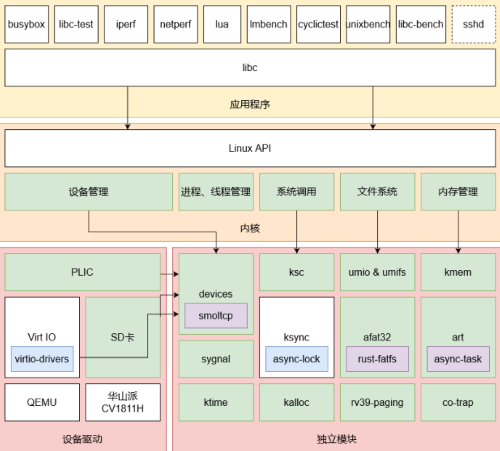
\includegraphics{figures/10-03-plntry.png}
    \caption{SD卡与K210接口}
\end{figure}

